\chapter{Hardware Compilation using SSA \Author{Pedro C. Diniz \andAuthor Philip Brisk}
}
\inputprogress
\graphicspath{{Figs/}{hardware_compilation/Figs/}{part4/hardware_compilation/Figs/}}
\label{chapter:hardware_compilation}
\abstract{
This chapter describes the use of SSA-based high-level 
program representation for the realization of the 
corresponding computation using hardware circuits. 
We begin by highlighting the benefits of using a compiler 
SSA-based intermediate representation in this hardware
mapping process using an illustrative example.
The following sections describe hardware translation 
schemes for the core hardware logic or data-paths of
hardware circuits. 
In this context we also outline several compiler 
transformations that benefit from the SSA-based
representation of a computation.
We conclude with a brief survey of various hardware
compilation efforts both from academia as well as
industry that have adopted SSA-based internal
representations.
%Finally, we conclude with several remarks on 
%research avenues in the use of SSA-based 
%representations for hardware compilation.
}

\renewcommand{\comment}[1]{}

\section{Brief history and overview}

Hardware compilation is the process by which a high-level 
language, or behavioral, description of a computation is 
translated into a hardware-based implementation i.e., a 
circuit expressed in a hardware design language such as 
VHDL or Verilog which
can be directly realized as an electrical (often digital) circuit. 
\comment{
Hardware compilation has a long rich history, since the 
early 70's, if not earlier, first as academic efforts in 
the context of VLSI design and later as high-level synthesis 
techniques successfully raised the level of abstraction of 
the computations the techniques were able to tackle. 
Reflecting its growing importance as productivity tools many 
of the high-level techniques have successfully migrated into 
commercial products for high-level hardware synthesis still 
used today in industry.}\\

While, initially, developers were forced to design hardware circuits using 
schematic-capture tools, high-level behavioral synthesis allowed them over 
the years to leverage the wealth of hardware-mapping and design exploration 
techniques to realize substantial productivity gains. 
As an example Figure~\ref{fig:Fig.4.1} illustrates these concepts
of hardware mapping for the computation expressed as
{\tt x = (a * b) - (c * d) + f}.
In figure~\ref{fig:Fig.4.1}(b) a graphical representation of a circuit 
that directly implements this computation is presented. 
Here there is a direct mapping of hardware operator such
as adders and multipliers to the operations in the computation. 
Values are stored in register and the entire computation lasts a 
single (albeit long) clock cycle. 
The input data values are stored in the input registers on the left and 
a clock cycle later the corresponding results of the computation are ready 
and saved in the output registers on the right-hand-side of the figure. 
Overall this direct implementation uses two multipliers, two adders/subtractors 
and six registers. 
The execution using this design implementation can use a very simple
control scheme, as it simply uses the data in the  input registers, waits
for a single clock cycle and stores the outputs of the operations in the
output registers. 
In figure~\ref{fig:Fig.4.1}(c) we depict a different implementation variant 
of the same computation, this time using nine registers and the same amount 
of adders and subtractors. The increased number of registers allows for the 
circuit to be clocked at higher frequency as well as to be executed in a 
pipelined fashion. 
Finally, in figure~\ref{fig:Fig.4.1}(d) we depict yet another possible 
implementation of the same computation but using a single multiplier operator. 
This last version allows for the reuse in time of the multiplier operator and 
required thirteen register as well as multiplexers to route the inputs to the 
multiplier in two distinct control steps. As it is apparent, the reduction of 
number of operators, in this particular case the multipliers carries a penalty 
on increased number of registers, 
multiplexers \footnote{A $2\times1$ multiplexor is a combinatorial circuit with 
two data inputs, a single output and a control input, where the control input 
selects which of the two data inputs is transmitted to the output. It can be 
viewed as a hardware implementation of the C programming language selection 
operator : {\tt out = (sel ? in1 : in2)}.} and increased complexity of the 
control scheme.\\

\begin{figure}[htbp]
\centering
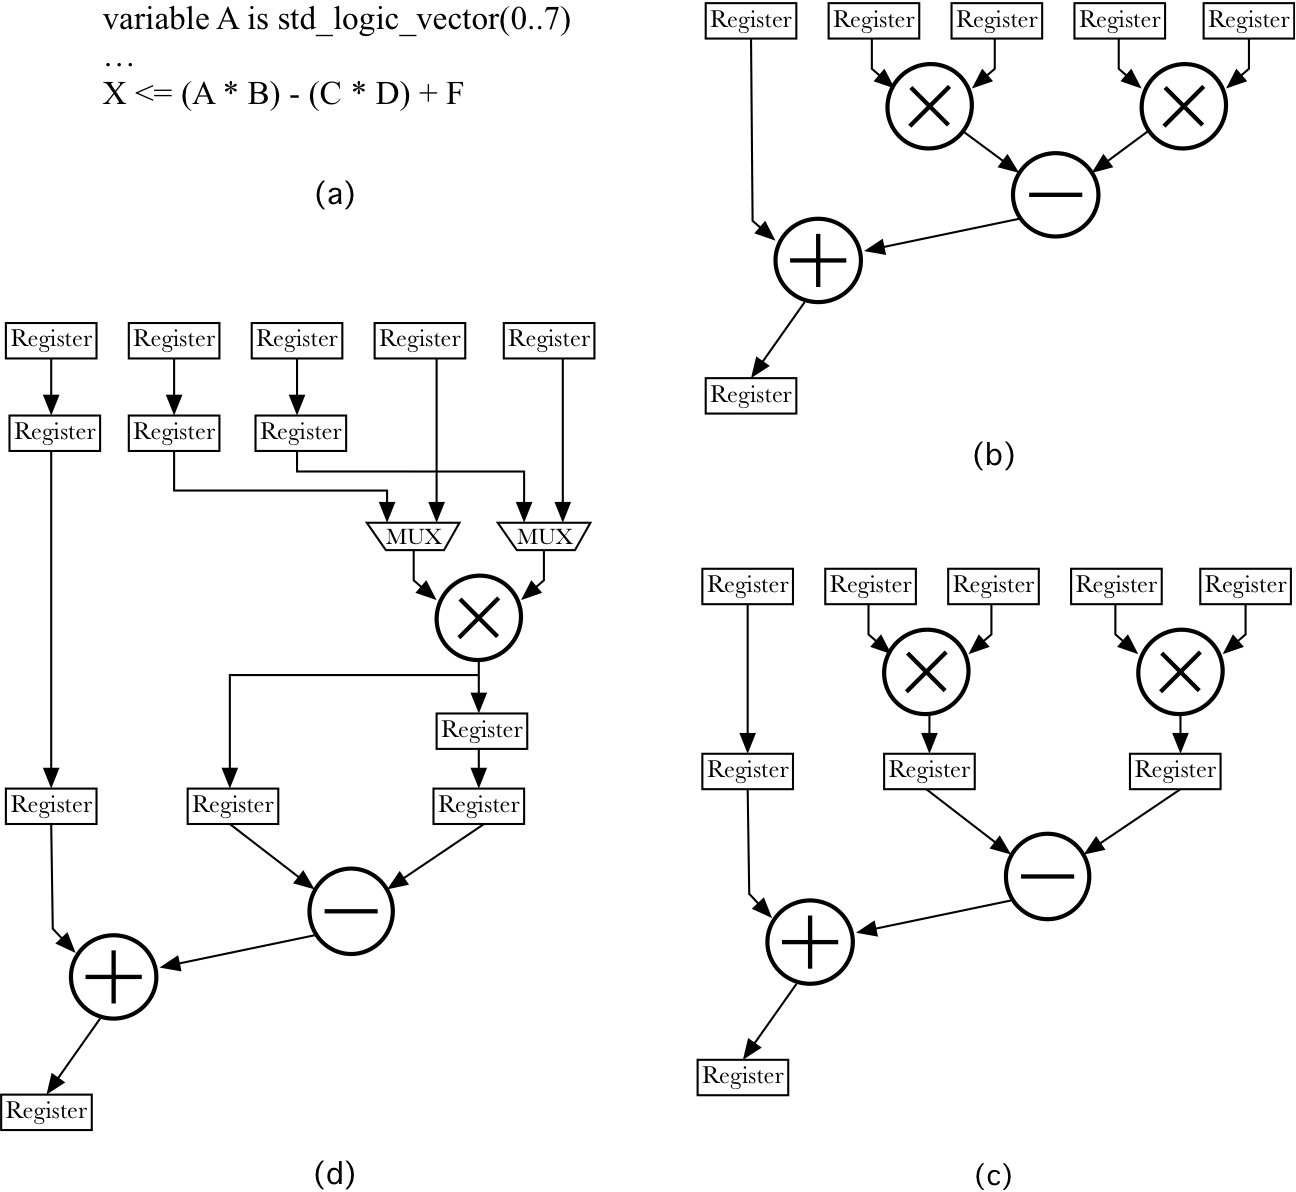
\includegraphics[scale=0.5]{Fig-4-1}
\caption{Variants of mapping a computation to hardware: High-level source 
code (a); a simple hardware design (b); pipelined hardware 
design (c) design sharing resources (d).} 
\label{fig:Fig.4.1}
\end{figure}

This example illustrates the many degrees of freedom in high-level
behavioral hardware synthesis. Synthesis techniques perform the
classical tasks of allocation, binding and scheduling of the various
operations in a computation given specific target hardware resources. 
For instance, a designer can use behavioral synthesis tools (e.g.,
Mentor Graphics's Monet$^{\textregistered}$) to automatically derive
an implementation for a computation as expressed in the example in
Figure~\ref{fig:Fig.4.1}(a) by declaring that it pretends to use a
single adder and a single multiplier automatically deriving an
implementation that resembles the one depicts in figure~\ref{fig:Fig.4.1}(d). 
The tool then derives the control scheme required to route the data from 
registers to the selected units so as to meet the designers' goals. 
\comment{
This approach thus allows designs to retain some control of the generated 
hardware design while relieving them from the low-level and error prone 
details of hardware synthesis and thus have increased tremendously the 
productivity of designers over previous schematic capture and structural 
design approaches\footnote{Structural design approach require designers 
to explicitly implement all the control structures such as 
Finite-State-Machines (FSM) and the corresponding control signals for 
maximum design control and clock rate control.}
}\\

Despite the introduction of high-level behavioral synthesis techniques in 
commercially available tools, hardware synthesis and thus hardware
compilation has never enjoyed the same level of success as traditional,
software compilation. 
Sequential programming paradigms popularized by programming
languages such as C/C++ and more recently by Java, allow
programmers to easily reason about program behavior as a
sequence of program memory state transitions. The underlying
processors and the corresponding system-level implementations
present a number of simple unified abstractions -- such as a
unified memory model, a stack, and a heap� that do not exist (and
often do not make sense) in customized hardware designs.\\

Hardware compilation, in contrast, has faced numerous obstacles
that have impeded its progress and generality. When developing
hardware solutions, designers must understand 
the concept of spatial concurrency 
\comment{(parallelism both in space and in time)}
that circuits do offer. Precise timing and synchronization between
distinct hardware components are key abstractions in hardware. 
Solid and robust hardware design implies a detailed understanding of 
the precise timing of specific operations, including I/O, that simply 
cannot be expressed in language such as C, C++, or Java; for this reason, 
alternatives, such as SystemC have emerged in 
recent years, which give the programmer considerably more control 
over these issues. 
The inherent complexity of hardware designs has hampered the development 
of robust synthesis tools that can offer high-level programming abstractions 
enjoyed by tools that target traditional architecture and software systems, 
thus substantially raising the barrier of entry for hardware designers in 
terms of productivity and robustness of the generated hardware solutions. 
At best, today hardware compilers can only handle certain subsets of 
mainstream high-level languages, and at worst, are limited to purely 
arithmetic sequences of operations with strong restrictions on control flow.\\

Nevertheless, the emergence of multi-core processing has led to the 
introduction of new parallel programming languages and parallel 
programming constructs that may be more amenable to hardware compilation 
than traditional languages and, similarly, abstractions such as a heap 
(e.g., pointer-based data structures) and a unified memory address space are 
proving to be bottlenecks with respect to effective parallel programming. 
For example, MapReduce, originally introduced by Google to spread parallel 
jobs across clusters of servers, has been an effective 
programming model for FPGAs; similarly, high-level 
languages based on parallel models of computation such as synchronous data 
flow, or functional single-assignment languages have 
also been shown to be good choices for hardware 
compilation.\\

Although the remainder of this chapter will be limited primarily to 
hardware compilation for imperative high-level programming languages
with  an obvious focus on SSA Form, many of the emerging parallel languages will 
retain sequential constructs, such as control-flow graphs, within a larger 
parallel framework. The extension of SSA Form, and SSA-like constructs, to 
these emerging languages, is an open area for future research; however, 
the fundamental uses of SSA Form for hardware compilation, as discussed 
in this chapter, are likely to remain generally useful.\\


\section{Why use SSA for hardware compilation?}

Hardware compilation, unlike its software counterpart, offers a spatially 
oriented computational infrastructure that presents opportunities that can 
leverage information exposed by the SSA representation. We illustrate the 
direct connection between SSA representation form and hardware compilation 
using the mapping of a computation example in Figure~\ref{fig:Fig.4.2}(a). 
Here the value of a variable {\tt v} depends on the control flow of 
the computation as the temporary variable {\tt t} can be assigned 
different values depending on the value of the {\tt p} predicate. 
The representation of this computation is depicted in 
Figure~\ref{fig:Fig.4.2}(b) where a \phifun is 
introduced to capture the two possible assignments to the temporary 
variable {\tt t} in both control branches of the {\tt if-then-else} 
construct.  Lastly, we illustrate in Figure~\ref{fig:Fig.4.2}(c) 
the corresponding mapping to hardware.\\

\begin{figure}[htbp]
\centering
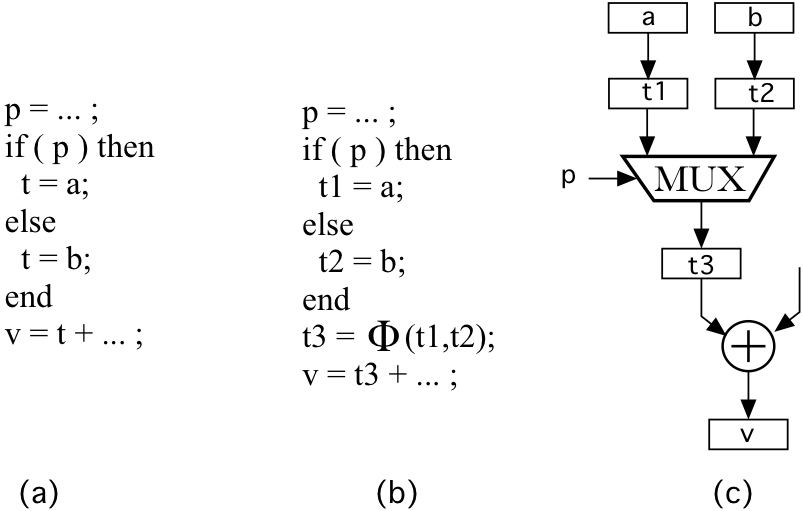
\includegraphics[scale=0.45]{Fig-4-2}
\caption{Basic hardware mapping using SSA representation.}
\label{fig:Fig.4.2}
\end{figure}

The basic observation is that the confluence of values for a given
program variable leads to the use of a \phifun.
This \phifun abstraction thus corresponds in terms
of hardware implementation of the insertion of a multiplexer logic circuit. 
This logic circuit uses the Boolean value of a control input to select which of its 
input's value is to be propagated to its output. The selection or control input of 
a multiplexer thus acts as a gated transfer of value that parallels the actions of 
an {\tt if-then-else} construct in software.\\

Equally important in this mapping to hardware is the notion that the computation 
in hardware can now take a spatial dimension. In the suggested hardware circuit 
in Figure~\ref{fig:Fig.4.2}(c) the computation derived from the statement in both 
branches of the {\tt if-then-else} construct can be evaluated concurrently by 
distinct logic circuits. After the evaluation of both circuits the multiplexer 
will define which set of values are used based on the value of its control 
input, in this case of the value of the computation associated with {\tt p}.\\

In a sequential software execution environment, the predicate {\tt p} 
would be evaluated  first, and then either branches of the {\tt if-then-else} construct would be evaluated, 
based on the value of p; as long as the register allocator is able to assign 
{\tt t1}, {\tt t2}, and {\tt t3} to the same register, then the \phifun 
is executed implicitly; if not, it is executed as a register-to-register copy. \\

There have been some efforts that could automatically convert the
sequential program above into a semi-spatial representation that
could obtain some speedup if executed on a VLIW type of processor. 
For example, if-conversion (See Chapter~\ref{chapter:if_conversion}) would convert the control dependency into 
a data dependency: statements from the {\tt if}- 
and {\tt else} blocks could be interleaved, as long as they do not
overwrite one another's values, and the proper result
(the \phifun) could be selected using a 
conditional-move instruction; however, in the worst case, this would 
effectively require the computation of both sides of the branch, rather 
than one, so it could actually lengthen the amount of time required to 
resolve the computation; in the spatial representation, in contrast, the 
correct result can be output as soon as two of the three inputs to the 
multiplexer are known ({\tt p}, and one of {\tt t1} or {\tt t2}, depending 
on the value of {\tt p}). \\

%%% need to fix sentences below.
When targeting a hardware platform, one advantage of the SSA
representation is that assigning a value to each scalar variable
exactly once makes the sequences of definitions and uses of
each variable both formal and explicit. 
A spatially-oriented infrastructure can leverage this information to perform 
the computation in ways that would make no sense in a traditional processor. 
For example, in an FPGA, one can use multiple registers in 
space and in time to hold the same variable, and even simultaneously assign 
distinct values to it; then, based on the outcome of specific predicates in 
the program, the hardware implementation can select the
appropriate register to hold the outcome of the computation. 
In fact, this is precisely what was done using a multiplexer in
the example above.\\

This example highlights the potential benefits of a SSA-based intermediate representation, when
targeting hardware architectures that can easily exploit spatial
computation, namely:\\
\begin{itemize}
\item Exposes the data dependences in each variable computation
by explicitly  incorporating into the representation each variable
{\em def-use} chains.  This allows a compiler to isolate the
specific values and thus possible registers that  contribute to
each of the assumed values of the variable. Using separate registers for disjoint live ranges, allows hardware generation
to  reduce the amount of resources in multiplexer circuits, for example.
\item Exposes the potential for the sharing of hardware register not only in 
time and but also in space providing insights for the high-level synthesis
steps of allocation, binding and scheduling.
\item Provides insight into control dependent regions where control 
predicates and thus the corresponding circuitry is identical and can
thus be shared. This aspect has been so far neglected but might
play an important role in the context of energy minimization. \\
\end{itemize}

While the Electronic Design Automation (EDA) community had for
several decades now exploited similar information regarding data
and control dependences for the generation of hardware circuits
from increasingly higher-level representations 
(e.g., Behavioral HDL), SSA makes these dependences
explicit in the intermediate representation  itself.
Similarly, the more classical compiler representations, using three-address 
instructions augmented with the {\em def-use} chains already exposes the data-flow 
information as for the SSA-based representation. The later however,
and as we will explore in the next section, facilitates the mapping and 
selection of hardware resources.\\


\section{Mapping a control-flow graph to hardware}
\comment{
We begin by describing the mapping to hardware of a computation
expressed as a sequence of three-address instructions\footnote{In
this context we assume 
the use of a simple imperative three address instructions of the form 
{\tt a = b $\oplus$ c} where {\tt a}, {\tt b}, and {\tt c} are scalar 
variables or registers and $\oplus$ is a generic two input operation. 
Simple generalization for single-input operators and array operators are 
possible and follow the same rationale.} in a basic block or a data flow 
and then evolve by describing how to combine in the mapping the hardware 
circuits derived from multiple basic blocks, first in a straight-forward 
but inefficient fashion and then exploiting the knowledge captured in the 
SSA representation.
}
In this section we are interested in hardware implementations 
or circuit that are spatial in nature and thus we do not address
the mapping to architectures such as VLIW (Very Long Instruction Word)
or Systolic Arrays. 
While these architectures pose very interesting and challenging issues,
namely scheduling and resource use, we are more interested in exploring
and highlighting the benefits of  SSA representation which, we believe, are
more naturally (although not exclusively) exposed in the context of spatial
hardware computations.\\

\subsection{Basic block mapping}
As a basic block is a straight-line sequence of three-address instructions, 
a simple hardware mapping approach consists in composing or evaluating
the operations in each instruction as a data-flow graph.
The inputs and outputs of the instructions are transformed into
registers\footnote{As a first approach these registers are virtual
and then after synthesis some of them are 
materialized to physical registers in a process similar to register 
allocation in software-oriented compilation.} connected by nodes in 
the graph that represent the operators. 
\comment{
Figure~\ref{fig:Fig.4.3} outline an algorithm that creates such a 
data-flow representation of the computation amenable to direct 
hardware synthesis. 
The algorithm sequentially evaluates each instruction, in a 
symbolic fashion maintaining a binding of the scalar variable
names to a register in the data-flow representation 
using the function {\tt mapNameToRegister}. 
Whenever no binding is found the algorithm uses the
function {\tt allocateRegister} to create
a new node in the data-flow representation 
that captures a value of a variable and thus
of a partial computation.
To assign the new value of a variable to a new hardware register
the algorithm uses the {\tt bindNameToRegister} function.
It then uses the function {\tt createComputationNode} to
create a representation of the computation with the registers
derived previously.\\
}

\comment{
\begin{figure}[htbp]
\centering
\begin{tabular}{c}
\begin{minipage}{4.5 in}
\begin{center}  
\parbox{4.5in}{
{\tt
\scriptsize
\begin{tabbing}
a\= a\= a\= a\= a\= a\= a\= a\=\kill
for each instruction i: z = x $\oplus$ y in basic block B do\\
\> rx = mapNameToRegister(x);\\
\> if(rx = nil) then\\
\>\> rx = allocateRegister(x);\\
\> end if\\
\> ry = mapNameToRegister(y);\\
\> if(ry = nil) then\\
\>\> ry = allocateRegister(y);\\
\> end if\\
\> rz = allocateRegister(z);\\
\> bindNameToRegister(rz, z);\\
\> createComputationNode(rz, rx, $\oplus$, ry);\\
end for\\
~\\
for all variables v in basic block B do\\
\> if (v is live at output of B) then\\
\>\> saveRegister(mapNametoRegister(v));\\
\> end if\\
end for
\end{tabbing}
}
}
\end{center}  
\end{minipage}
\end{tabular}
\normalsize
\caption{Basic-Block hardware mapping algorithm.}
\label{fig:Fig.4.3}
\end{figure}

As a last step the algorithm saves the registers corresponding
to the live variables at the output of the basic block. These registers
will be used to communicate the values of the live variables to
subsequent hardware circuits, either by having their values copied
to a local storage or directly connected via wires to other hardware
circuits (see description in section~\ref{sec:cfg_mapping}).
}
As a result of the "evaluation" of the instructions in the basic
block this algorithm constructs a hardware circuit
that has as input registers that will hold the values of the input
variables to the various instructions and will have as outputs
registers that hold only variables that are live outside
the basic block. \\

\subsection{Basic control-flow graph mapping}
\label{sec:cfg_mapping}

One can combine the various hardware circuits corresponding
to a control-flow graph in two basic approaches, respectively,
{\em spatial} and {\em temporal}. 
The spatial form of combining the hardware circuits consists 
in laying out the various circuits spatially by connecting 
variables that are live at the output of a basic block, 
and therefore the output registers of the 
corresponding hardware circuit, to the registers that 
will hold the values of those same variables in subsequents 
hardware circuits of the basic blocks that execute 
in sequence.

In the temporal approach the hardware circuits corresponding
to the various CFG basic blocks are not directly interconnected.
Instead their input and output registers are connected via dedicated
buses to a local storage module. An execution controller "activates"
a basic block or a set of basic blocks by transferring data between
the storage and the input registers of the hardware circuits to be
activated. Upon execution completion the controller transfers the
data from the output registers of each hardware circuit to the storage module.
These data transfers do not need necessarily to be carried out
sequentially but instead can leverage the aggregation of the
outputs of each hardware circuits to reduce transfer
time to and from the storage module via dedicated wide buses.\\

\begin{figure}[htbp]
\centering
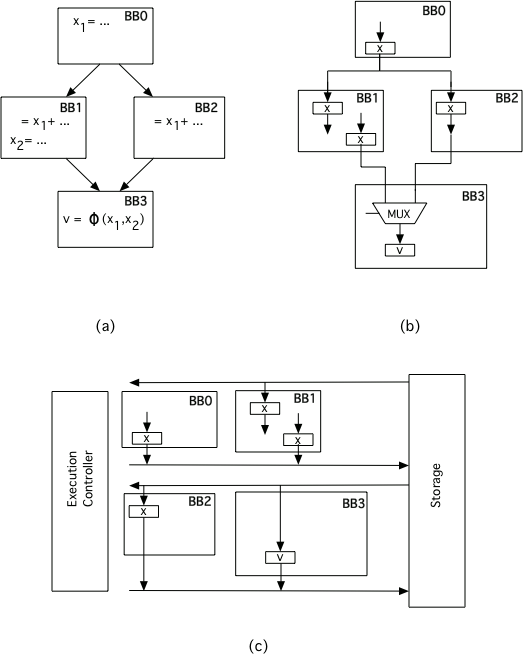
\includegraphics[scale=0.4]{Fig-4-4}
\caption{Combination of hardware circuits for multiple basic blocks. 
CFG representation (a); Spatial mapping (b); Temporal mapping (c).}
\label{fig:Fig.4.4}
\end{figure}

The temporal approach described above is well suited for the 
scenario where the target architecture does not have sufficient
resources to simultaneously implement the hardware circuits 
corresponding to all basic blocks of interest as it trades off 
execution time for hardware resources.\\

In such a scenario, where hardware resources are very limited
or the hardware circuit corresponding to a set of basic blocks is 
exceedingly large, one could opt for partitioning a basic block or
set of basic blocks into smaller blocks until the space constraints
for the realization of each hardware circuit are met. In reality
this is the common approach in every processor today. 
It limits the hardware resources to the resources required
for each of the ISA instructions and schedules them in time
at  each step saving the state (registers)
that were the output of the previous instruction.
The computation thus proceed as described above by saving
the values of the output registers of the hardware circuit
corresponding to each smaller block.\\

These two approaches, illustrated in Figure~\ref{fig:Fig.4.4}, can 
obviously be merged in a hybrid implementation. As they lead to distinct
control schemes for the orchestration of the execution of
computation in hardware, their choice depends heavily
on the nature and granularity of the target hardware architecture. 
For fine-grain hardware architectures such as FPGAs~\footnote{Field-Programmable Gate Arrays are layers of two dimensional topology integrated circuits designed to be configurable after manufacturing} a spatial
mapping can be favored, for coarse-grain architectures a
temporal mapping is common.\\

While the overall execution control for the temporal mapping
approach is simpler, as the transfers to and from the storage module are done upon the transfer of control between hardware circuits,
a spatial mapping approach makes it more amenable to 
take advantage of pipelining execution techniques and 
speculation~\footnote{Speculation is also possible in 
the temporal mode by activating the inputs and execution 
of multiple hardware blocks and is only limited by the 
available storage bandwidth to restore the input context 
in each block which in the spatial approach is trivial.}.
The temporal mapping approach can be, however, 
area-inefficient, as often only one basic block will
execute at any point in time. 
This issue can, nevertheless, be mitigated by exposing
additional amounts of instruction-level parallelism by
merging multiple basic blocks into a single {\em hyper-block}
and combining this aggregation with loop unrolling. 
Still, as these transformations and their combination, can
lead to a substantial increase of the required hardware
resources, a compiler can exploit resource sharing
between the hardware units  corresponding to distinct
basic blocks to reduce the pressure on resource
requirements and thus lead to feasible hardware
implementation designs. 
As these optimizations are not specific to the SSA representation, 
we will not discuss them further here. \\

%For a power consumption perspective, 
%however the temporal mapping approach,
%allows for a simpler selectivity of which
%circuits to momentarily shut-down.

\subsection{Control-flow graph mapping using SSA}
\label{sec:cfg_ssa_mapping}

In the case of the spatial mapping approach,  the SSA form plays an 
important role in the minimization of multiplexers and thus
in the simplification of the corresponding data-path logic
and execution control.\\

%The naive use of multiplexers whenever control-flow paths merge is, 
%however, in many cases unnecessary. 
Consider the illustrative example in Figure~\ref{fig:Fig.4.5}(a).
Here basic block {\tt BB0} defines a value for the variables {\tt x}
and {\tt y}. One of the two subsequent basic blocks {\tt BB1} 
redefines the value of {\tt x} whereas the other basic block
{\tt B2} only reads them.\\

A naive implementation based exclusively on {\em live} variable analysis
would use for both variables {\tt x} and {\tt y} multiplexers to merge their
values as inputs to the hardware circuit implementing basic block {\tt BB3}
as depicted in Figure~\ref{fig:Fig.4.5}(b). 
As can be observed, however, the SSA-form representation captures
the fact that such a multiplexer is only required for variable {\tt x}.
The value for the variable {\tt y} can be propagated either from the
output value in the hardware circuit for basic block {\tt BB0} (as shown
in Figure~\ref{fig:Fig.4.5}(c)) or from any other register that has
a valid copy of the {\tt y} variable.
The direct flow of the single definition point to all its uses, across
the hardware circuits corresponding to the various basic blocks in
the SSA form thus allows a compiler to use the minimal number of
multiplexer strictly required\footnote{Under the scenarios of a spatial
mapping and with the common disclaimers about static control-flow
analysis.}.\\

\begin{figure}[htbp]
\centering
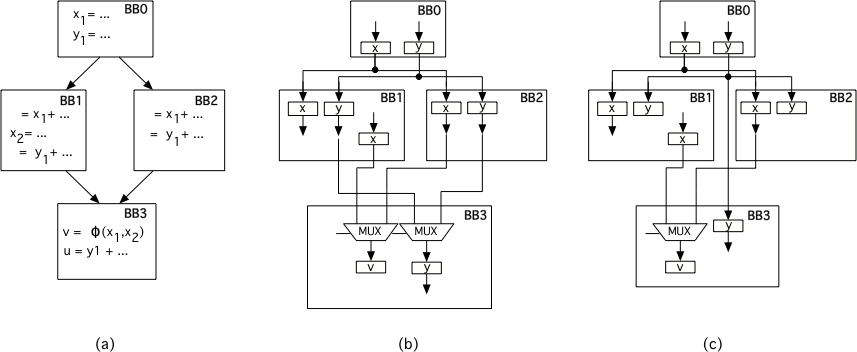
\includegraphics[scale=0.4]{Fig-4-5}
\caption{Mapping of variable values across hardware circuit
using spatial mapping;  CFG in SSA form (a); naive hardware
circuit using live variable information for multiplexer placement (b);
hardware circuit using \phifun for multiplexer placement (c).}
\label{fig:Fig.4.5}
\end{figure}

An important aspect regarding the implementation of a multiplexer 
associated with a \phifun is the definition and evaluation 
of the predicate associated with each multiplexer's control (or
selection) input signal.
In the basic SSA representation the selection predicates are
not explicitly defined, as the execution of each \phifun
is implicit when the control flow reaches it. 
When mapping a computation the \phifun to hardware,
however, one has to clearly define which predicate to use to be
included part of the hardware logic circuit that defines the value
of the multiplexer circuit's selection input signal. 
The Gated-SSA form previously described in Chapter~\ref{chapter:vsdg} of the SSA form
explicitly captures the necessary information in the representation. 
As the variable name associated with each gating predicate fulfills the referential transparency as any  SSA variable, 
this variant of the SSA form is particularly useful for hardware synthesis. 
The generation of the hardware circuit simply uses the 
register that holds the corresponding variable's version value of the predicate,
as opposed
to the base name of the variable as this might have been assigned a
value that does not correspond to the actual value used in the gate.
Figure~\ref{fig:Fig.4.6} illustrates an example of a mapping using the
information provided by the Gated-SSA form.\\

\begin{figure}[htbp]
\centering
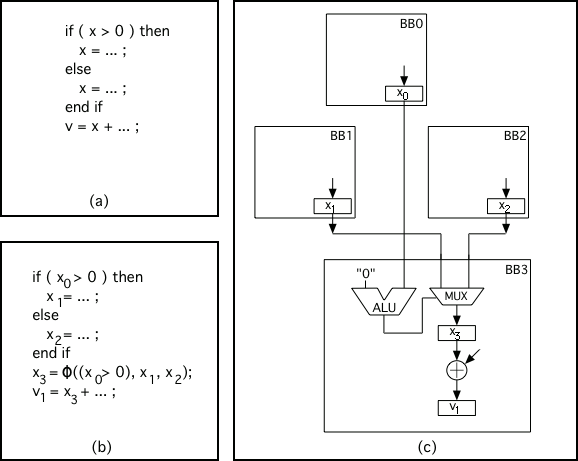
\includegraphics[scale=0.375]{Fig-4-6}
\caption{Hardware generation example using Gated-SSA form;\newline (a) original 
code; (b) Gated-SSA representation; (c) hardware circuit implementation 
using spatial mapping.}
\label{fig:Fig.4.6}
\end{figure}
%TODO: use the gamma notation here instead

When combining multiple predicates in the Gated-SSA form it is often
desirable to leverage the control-flow representation in the form of the
Program Dependence Graph (PDG) described in Chapter~\ref{chapter:vsdg}.
In this representation, basic blocks
that share common execution predicates (i.e., both execute under
the same predicate conditions) are linked to the same {\em region} 
nodes. Nested execution conditions are easily
recognized as the corresponding nodes are hierarchically organized
in the PDG representation.
As such, when generating code for a given basic block an algorithm
will examine the various region nodes associated with a given basic
block and compose (using AND operators) the outputs of the logic 
circuits that implementat the predicates associated with these nodes.
If an hardware circuit already exists for the same predicate, the 
implementation simply reuses its output signal.
Otherwise, creates a new hardware circuit.
This lazy code generation and predicate composition achieves the
goal of hardware circuit sharing as illustrated by the example in 
Figure~\ref{fig:Fig.4.7} where some of the details were omitted for
simplicity.\\

\begin{figure}[htb]
\centering
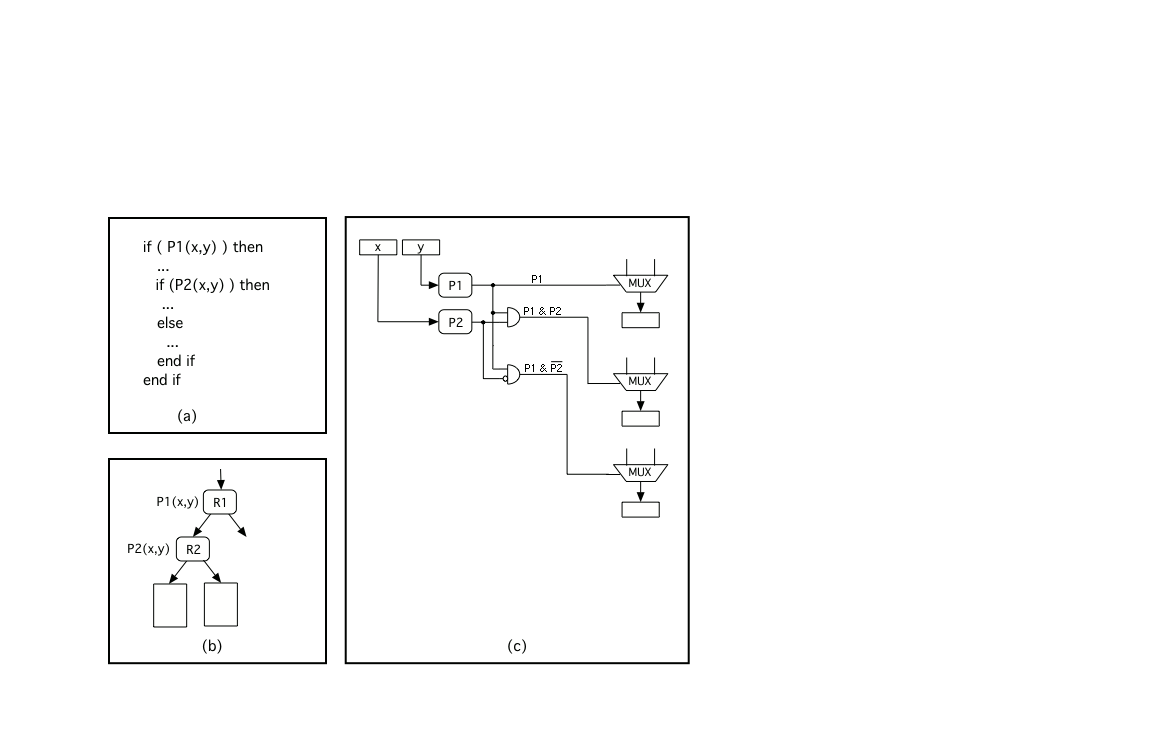
\includegraphics[scale=0.35]{Fig-4-7}
\caption{Use of the predicates in region nodes of the PDG for mapping 
into the multiplexers associated with each \phifun; a) source code; b)
the PDG representation skeleton; c) outline of hardware design implementation.}
\label{fig:Fig.4.7}
\end{figure}


\subsection{$\phi$-function and multiplexer optimizations}

We now describe a set of hardware-oriented transformations that can 
be applied to improve the amount of hardware resources devoted to 
multiplexer implementation.
Although these transformations are not specific to the mapping of
computations to hardware, the explicit representation
of the selection constructs in SSA makes it very natural to map and
therefore manipulate/transform the resulting hardware circuit
using multiplexer. Other operations in the intermediate 
representation (e.g., predicated instructions) can also yield
multiplexers in hardware without the explicit use of SSA Form.\\

A first transformation is motivated by a well-known result in computer 
arithmetic: integer addition scales with the number of operands. 
Building a large unified k-input integer addition circuit is more
efficient than adding k integers two at a time. 
Moreover, hardware multipliers naturally contain multi-operand adders 
as building blocks: a partial product generator (a layer of AND gates) 
is followed by a multi-operand adder called a {\em partial product reduction tree}. 
For these reasons, there have been several efforts in recent years to 
apply high-level algebraic transformations to source code
with the goal of merging multiple addition operations with
partial product reduction trees of multiplication operations.
The basic flavor of these transformations is to push the 
addition operators toward the outputs of a data-flow graph, so that 
they can be merged at the bottom. Example of these transformations 
that use multiplexers are depicted in Figure~\ref{fig:Fig.4.8}(a,b). 
In the case of Figure~\ref{fig:Fig.4.8}(a) the transformation
leads to the fact that an addition is always executed unlike in
the original hardware design. 
Figure~\ref{fig:Fig.4.8}(c) depicts a similar transformation that 
merges two multiplexers sharing a common input, while exploiting
the commutative property of the addition operator.
The SSA-based representation facilitates these transformations
as it explicitly indicates which values, and thus by tracing backwards
in the representation, are involved in the computation of the corresponding
values. For the example in Figure~\ref{fig:Fig.4.8}(b) the compiler
would quickly detect {\tt a} as a common variables in the two 
expressions associated with the \phifun.\\

A second transformation that can be applied to multiplexers is 
specific to FPGA whose basic building block consists of a k-input
lookup table (LUT) logic element which can be programmed to 
implement any k-input logic function.
For example, a 3-input LUT (3-LUT) can be programmed to
implement a multiplexer with two data inputs and one selection
bit; similarly, a 6-LUT can be programmed to implement a multiplexer
with four data inputs and two selection bits. 
In particular, many FPGAs devices are organized using 4-LUTs, 
which are too small to implement a multiplexer with four data inputs,
but leave one input unused when implementing multiplexers with
two data inputs. These features can be explored to reduce the number 
of 4-LUTs required to implement a tree of multiplexers.\\

\begin{figure}[thbp]
\centering
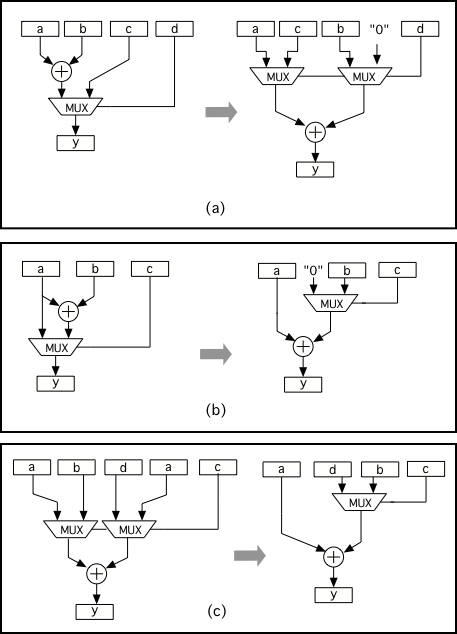
\includegraphics[scale=0.5]{Fig-4-8}
\caption{Multiplexer-Operator transformations: juxtapose the positions of
a multiplexer and an adder (a,b); reducing the number of multiplexers
placed on the input of an adder (c).}
\label{fig:Fig.4.8}
\end{figure}


\subsection{Implications of using SSA-form in floor-planing}

For spatial oriented hardware circuits, moving a \phifun
from one basic block to another can alter the length of the wires
that are required to transmit data from the hardware circuits
corresponding to the various basic blocks. 
As the boundaries of basic blocks are natural 
synchronization points, where values are captured in 
hardware registers, the length of wires dictate the maximum
allowed hardware clock rate for synchronous designs. 
We illustrate this effect via an example as depicted in 
Figure~\ref{fig:Fig.4.9}.
In this figure each basic block is mapped to a distinct hardware
unit, whose spatial implementation is approximated by a rectangle. 
A floor-planning algorithm must place each of the units in 
a two-dimensional plane while ensuring that no two units overlap. 
As can be seen in Figure~\ref{fig:Fig.4.9}(a) placing the block 5 on the 
right-hand-side of the plane will results in several mid-range 
and one long-range wire connections. However, placing block 5 
at the center of the design will virtually eliminate all 
mid-range connections as all connections corresponding to 
the transmission of the values for variable {\tt x} are now 
next-neighboring connections.\\

\begin{figure}[thbp]
\centering
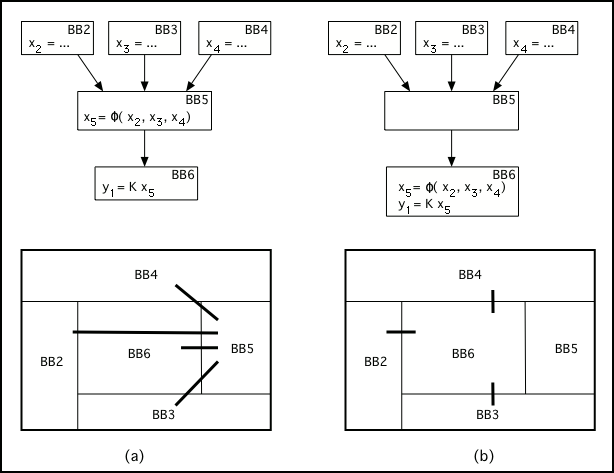
\includegraphics[scale=0.4]{Fig-4-9}
\caption{Example of the impact of \phifun movement in
reducing hardware wire length.}
\label{fig:Fig.4.9}
\end{figure}

As illustrated by this example, moving a multiplexer from one hardware 
unit to another can significantly change the dimensions of the resulting 
unit, which is not under the control of the compiler. Changing the 
dimensions of the hardware units fundamentally changes the placement 
of modules, so it is very difficult to predict whether moving a 
\phifun will actually be beneficial. For this reason, compiler 
optimizations that attempt to improve the physical layout must be 
performed using a feedback loop so that the results of the 
lower-level CAD tools that produce the layout can be reported 
back to the compiler.\\

%\section{Further readings}
\section{Existing SSA-based hardware compilation efforts}

Several research projects have relied on SSA-based intermediate representation 
that leverage control- and data-flow information to exploit fine grain parallelism. 
Often, but not always, these efforts have been geared towards mapping computations 
to fine-grain hardware structure such as the ones offered by FPGAs.\\

The standard approach followed in these compilers has been to 
translate a high-level programming language such as Java in 
the case of the Sea Cucumber~\cite{Tripp:FPL02} compiler or 
C in the case of the ROCCC~\cite{Najjar:ROCCC08} to sequences 
of intermediate instructions. These sequences are then organized 
in basic blocks that compose the control-flow graph (CFG). 
For each basic block a data-flow graph (DFG) is typically extracted 
followed by conversion in to SSA representation, possibly using 
predicates associated with the control flow in the CFG thus 
explicitly using Predicated SSA representation 
(PSSA~\cite{Carter:PACT99,deFerriere:SCOPES07,Stoutchinin:MICRO01}).\\

As an approach to increase the potential amount of exploitable 
instruction-level parallelism (ILP) at the instruction level, 
many of these efforts (as well as others such as the earlier 
Garp compiler~\cite{Callahan:Computer00}) restructure the CFG 
into hyper-blocks~\cite{Mahlke:Micro92}. 
An hyper-block consists on a single-entry multi-exit regions derived from the 
aggregation of multiple basic blocks thus serializing longer sequences of 
instruction. As not all instructions are executed in a hyper-block (due to 
early exit of a block), hardware circuit implementation must rely on predication 
to exploit the potential for additional ILP. \\

The CASH compiler~\cite{Budiu:FPL02} uses an augmented predicated SSA
representation with tokens to explicitly express synchronization and handle 
{\em may-dependences} thus supporting speculative  execution. 
This fine-grain synchronization mechanism is also used to serialize 
the execution of consecutive hyper-blocks, thus greatly simplifying 
the code generation.\\

{\bf I moved all the references found in the main body here. Please reorganize it.}
Put the reference for VHDL~\cite{VHDLBook}, Verilog~\cite{VerilogBook}, SystemC~\cite{SystemC:ISSS01}.

I guess a sentence summarizing what VHDL is would be helpful.

Add a reference for Mentor Graphics's if you think this is appropriate.

The following section taken from the main body contains many references that I removed. Might be put it here: {\em 
For example, MapReduce, originally introduced by Google to spread parallel 
jobs across clusters of servers~\cite{Dean:CACM08}, has been an effective 
programming model for FPGAs~\cite{Yeung:FCCM08}; similarly, high-level 
languages based on parallel models of computation such as synchronous data 
flow~\cite{Lee:ProcIEEE87}, or functional single-assignment languages have 
also been shown to be good choices for hardware 
compilation~\cite{Hormati:CASES08,Hagiescu:DAC09,SAC:IJS02}.}

I removed this citation~\cite{Allen:POPL83} concerning if-conversion and cross referred to the if-conversion chapter instead. Can be put here if you feel this is necessary.

Removed the reference for VLIW architecture~\cite{CompilingVLIWBook} and for Systolic Arrays~\cite{CompilingSystolicArraysBook}. Please insert it here if appropriate.

Removed in the Section Basic CFG Mapping the references~\cite{Hormati:CASES08,Kaplan:DAC03}.

I did not see any reference for FPGA that you talk about in the Basic CFG mapping section. I think you should give one and summaries in a sentence what FPGA is???

Removed this citation given for resource sharing in section Basic CFG mapping~\cite{Memik:DAC03}).

Removed the reference~\cite{Tu-SC95} about gated-SSA in section SSA based CFG mapping.

Removed the reference to the PDG~\cite{Ferrante-TOPLAS87}. 

Removed the reference associated to the following sentence: {\emph Building a large unified k-input integer addition circuit is more
efficient than adding k integers two at a time~\cite{Stelling98,Wallace64}. }

Removed the reference associated with the following sentence: {\emph Figure~\ref{fig:Fig.4.8}(c) depicts a similar transformation that 
merges two multiplexers sharing a common input, while exploiting
the commutative property of the addition operator~\cite{Verma08}.}

Removed the reference associated with the following sentence: {\emph These features can be explored to reduce the number 
of 4-LUTs required to implement a tree of multiplexers~\cite{Nancekievill05}.}

Removed the reference~\cite{Kaplan:DAC03} on the section of Floor planing.
